\begin{section}{Heurística constructiva}
		\begin{subsection}{Explicación}
			Como primera heurística, en este caso constructiva, desarrollamos un algoritmo goloso para resolver el problema \texttt{MAX-CLIQUE} de manera aproximada. El algoritmo parte del vértice de mayor grado en el grafo. En cada paso, agrega a la clique el vértice adyacente (al último agregado) de mayor grado que sea adyacente a todos los vértices en la clique obtenida hasta el momento. Este procedimiento se repite hasta que no se puedan agregar más vértices a la clique. (Figura \ref{fig:seguimiento_constructivo})
			
			% --- Figura seguimiento algoritmo constructivo ---
			\begin{figure}[H]
				\centering
		    	\includegraphics[scale=0.5]{constructivo/seguimiento.eps}
			    \caption{Ejemplo de la heurística constructiva}
			    \label{fig:seguimiento_constructivo}
			\end{figure}
			
			[REDACTAR MEJOR] -- Por qué este criterio goloso? Se eligió este criterio para el algoritmo goloso pensando en la posibilidad de que el vértice con mayor grado está en la clique máxima, y los nodos adyacentes de mayor grado son los que la forman.
			
			Desventajas: si la clique máxima no incluía al vértice de mayor grado, la solución puede ser muy mala.
			
			Al ser un algoritmo goloso, en este problema como en tantos otros, no devuelve necesariamente el óptimo. Particularmente, la clique está condicionada al vértice de mayor grado, y no necesariamente la solución óptima lo contiene.\VSP
		\end{subsection}
		\begin{subsection}{Detalles de la implementación}
			[REDACTAR MEJOR]
			El mismo funciona de la siguiente manera:

			Sea $grados$ un arreglo de tamaño $n$, donde $n$ es la cantidad de vértices del grafo. En cada posición $j\; \forall 	1\leq j \leq n$ del arreglo está el grado correspondiente al vértice $j$.
			Para construir una clique ordenamos $grados$ en forma decreciente. El primer vértice del arreglo, es decir, el de mayor grado del grafo se considera parte de la solución final del algoritmo.
			Para completar la clique recorremos $grados$ en forma completa, y cada vértice que forma un completo con la solución parcial se agrega a la misma.
			Al terminar de recorrer $grados$ el algoritmo termina siendo la solución parcial, el resultado final.

			A continuación, se muestra el pseudocódigo del algoritmo de heurística constructiva.\\

			\begin{pseudo}
				\func{constructivo}{matriz\_adyacencia,n}
				\tab $grados[n] \leftarrow ordenar\_grados(matriz\_adyacencia)$\\
				\tab $solucion[n]$\\
				\tab $solucion[0] \leftarrow grados[0]$\\
				\tab $tamanyo \leftarrow 1$\\
				\tab $\FOR i \TO n$\\
				\tab \tab $\IF \neg solucion[i]$\\
				\tab \tab \tab $completo \leftarrow forma\_completo(solucion,i,matriz\_adyacencia)$\\
				\tab \tab \tab $\IF completo$\\
				\tab \tab \tab \tab $solucion[i] \leftarrow true$\\
				\tab \tab \tab \tab $tamanyo \leftarrow tamanyo + 1$\\
				\RET $tamanyo$\\
			\end{pseudo}

			\begin{itemize}
				\item \texttt{ordenar\_grados: } En la implementación, el arreglo $grados$ es de tipo tupla donde la primer componente representa el vértice y la segunda el grado. Dicho arreglo está ordenado según la segunda componente en forma decreciente. Lo ordenamos con el algoritmo de Quick Sort de $STL$.
				
				Para setear el grado de un vértice $i$ tenemos un contador inicializado en $cero$. Recorremos la columna de la matriz de adyacencia correspondiente a dicho vértice e incrementamos el contador por cada posición $(i,j)$ igual $uno$.
				\item \texttt{forma\_completo: } Para saber si agregar un vértice $v$ determina una solución al problema debemos verificar que forme un completo con los vértices ya incluídos. Para esto recorremos todos los vértices del grafo y para cada uno que pertenezca a la solución parcial chequeamos que sea adyacente a $v$. Si esto ocurre podemos agregar el vértice $v$ y agrandar la clique.
			\end{itemize}
		\end{subsection}
		\begin{subsection}{Complejidad temporal}
			El algoritmo empieza inicializando el arreglo $grados$ lo que tiene un costo de $n^2$ ya que para cada vértice recorre la columna correspondiente en la matriz de adyacencia (diseñada como un arreglo de arreglos).
			
			Como mencionamos anteriormente, $grados$ es ordenado con un algoritmo de QuickSort dado por la librería estándar de C++. El costo del algoritmo es $n^2$.
			
			El algoritmo constructivo, una vez realizadas las operaciones antes mencionadas, entra a un ciclo $for$ que itera desde $0$ hasta $n$. En cada iteración, debe en primera instancia, analizar una guarda $if$. De ser $falsa$, procederá a la siguiente iteración del ciclo (teniendo así costo constante). De ser $verdadera$ (es decir, el vértice $i$ no forma parte de la solución parcial), analizará si puede formar una nueva clique mayor, ahora con el vértice $i$ (en nuestro pseudo-código, la función $forma\_completo$ es la encargada de analizarlo). Con el resultado de $forma\_completo$ la iteración del $for$ principal analiza una guarda $if$ más de costo constante (en el peor caso realiza dos asignaciones y una suma). Sabemos entonces que el costo de este ciclo será como mínimo $n$. Analizaremos a continuación el costo de $forma\_completo$, para concluir el costo total del algoritmo.
			
			$forma\_completo$, como ya dijimos antes, recorre todos los vértices del grafo analizando que, los vértices que pertenecen a la solución parcial, sean adyacentes al que queremos agregar. Esta función itera por todos los vértices del grafo, teniendo así un costo lineal en función de la cantidad de vértices.
			
			Como el ciclo $for$ del algoritmo constructivo, en el peor caso, llamaría una vez por cada una de las $n$ iteraciones a la función $forma\_completo$, el costo del ciclo entonces es cuadrático en función de la cantidad de vértices.
			
			Tenemos entonces en el algoritmo constructivo, la inicialización del arreglo con costo de $n^2$, el QuickSort de STL, costo $n^2$ y el ciclo $for$ también con costo a lo sumo cuadrático. La complejidad asintótica del problema viene dada entonces por la suma de las complejidades anteriormente descriptas. Podemos afirmar que el costo es \Ode{n^2}, ya que \Ode {n^2 + n^2 + n^2} = \Ode{3*n^2} = \Ode{n^2}.
			
		\end{subsection}

\end{section}

